\section{Network emulation environment} \label{sec:SDNNetSim}
The Mininet environment \cite{Mininet} has been used to emulate a SDN network to validate the methodology that will be presented in terms of prediction accuracy and control performance. This software runs a collection of virtual network elements (i.e. end-hosts, switches, routers, and links) on a single Linux kernel using lightweight virtualization. 
%To test the effectiveness of the realized controller a simulated network has been programmed using the Mininet environment as a network emulation orchestration system. This software runs a collection of end-hosts, switches, routers, and links on a single Linux kernel by using lightweight virtualization to make a single system look like a complete network. Mininet's virtual objects emulate real SDN network devices. It is usually possible to create a Mininet network that resembles a hardware network, or a hardware network that resembles a Mininet network, and to run the same binary code and applications on either platform.
To generate traffic the D-ITG generator \cite{Avallone2004, Botta2012, Botta2013} has been used.

\begin{figure}[htb!]
	\centering
	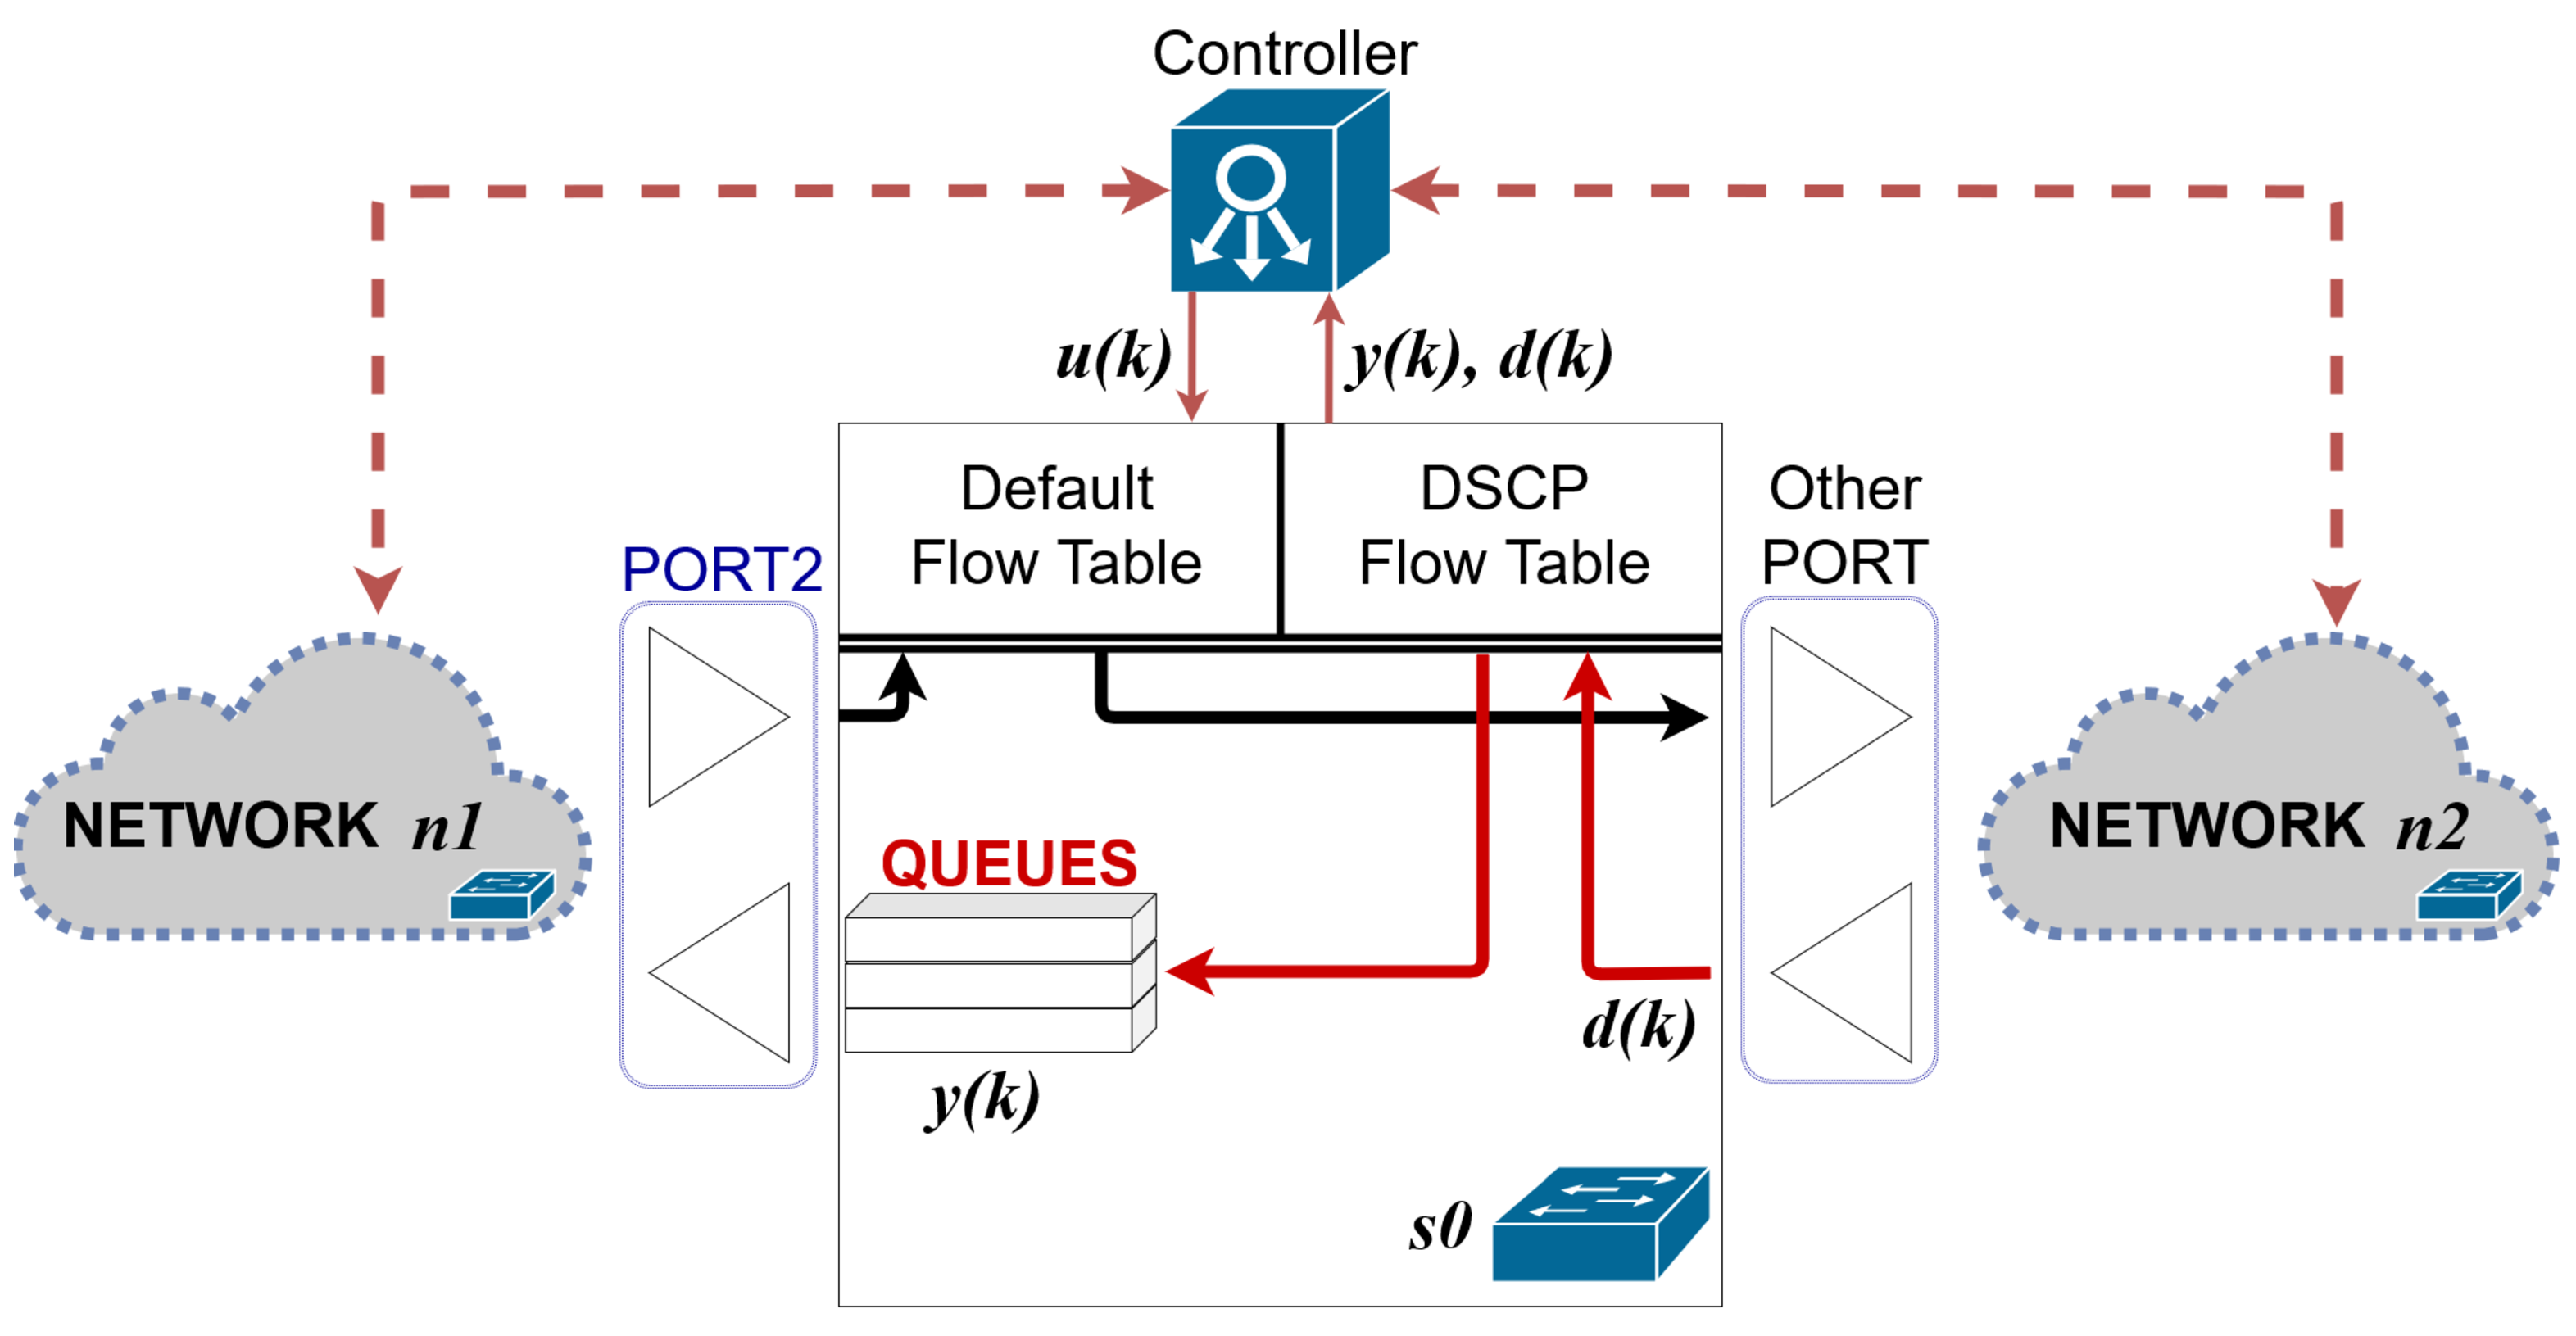
\includegraphics[keepaspectratio,width=\columnwidth]{figure/SDN_net_EPS.eps}
	\caption{Mininet emulated network architecture.}
	\label{fig:{Network}}
\end{figure}
%\begin{figure}[tb!]
%	\centering
%	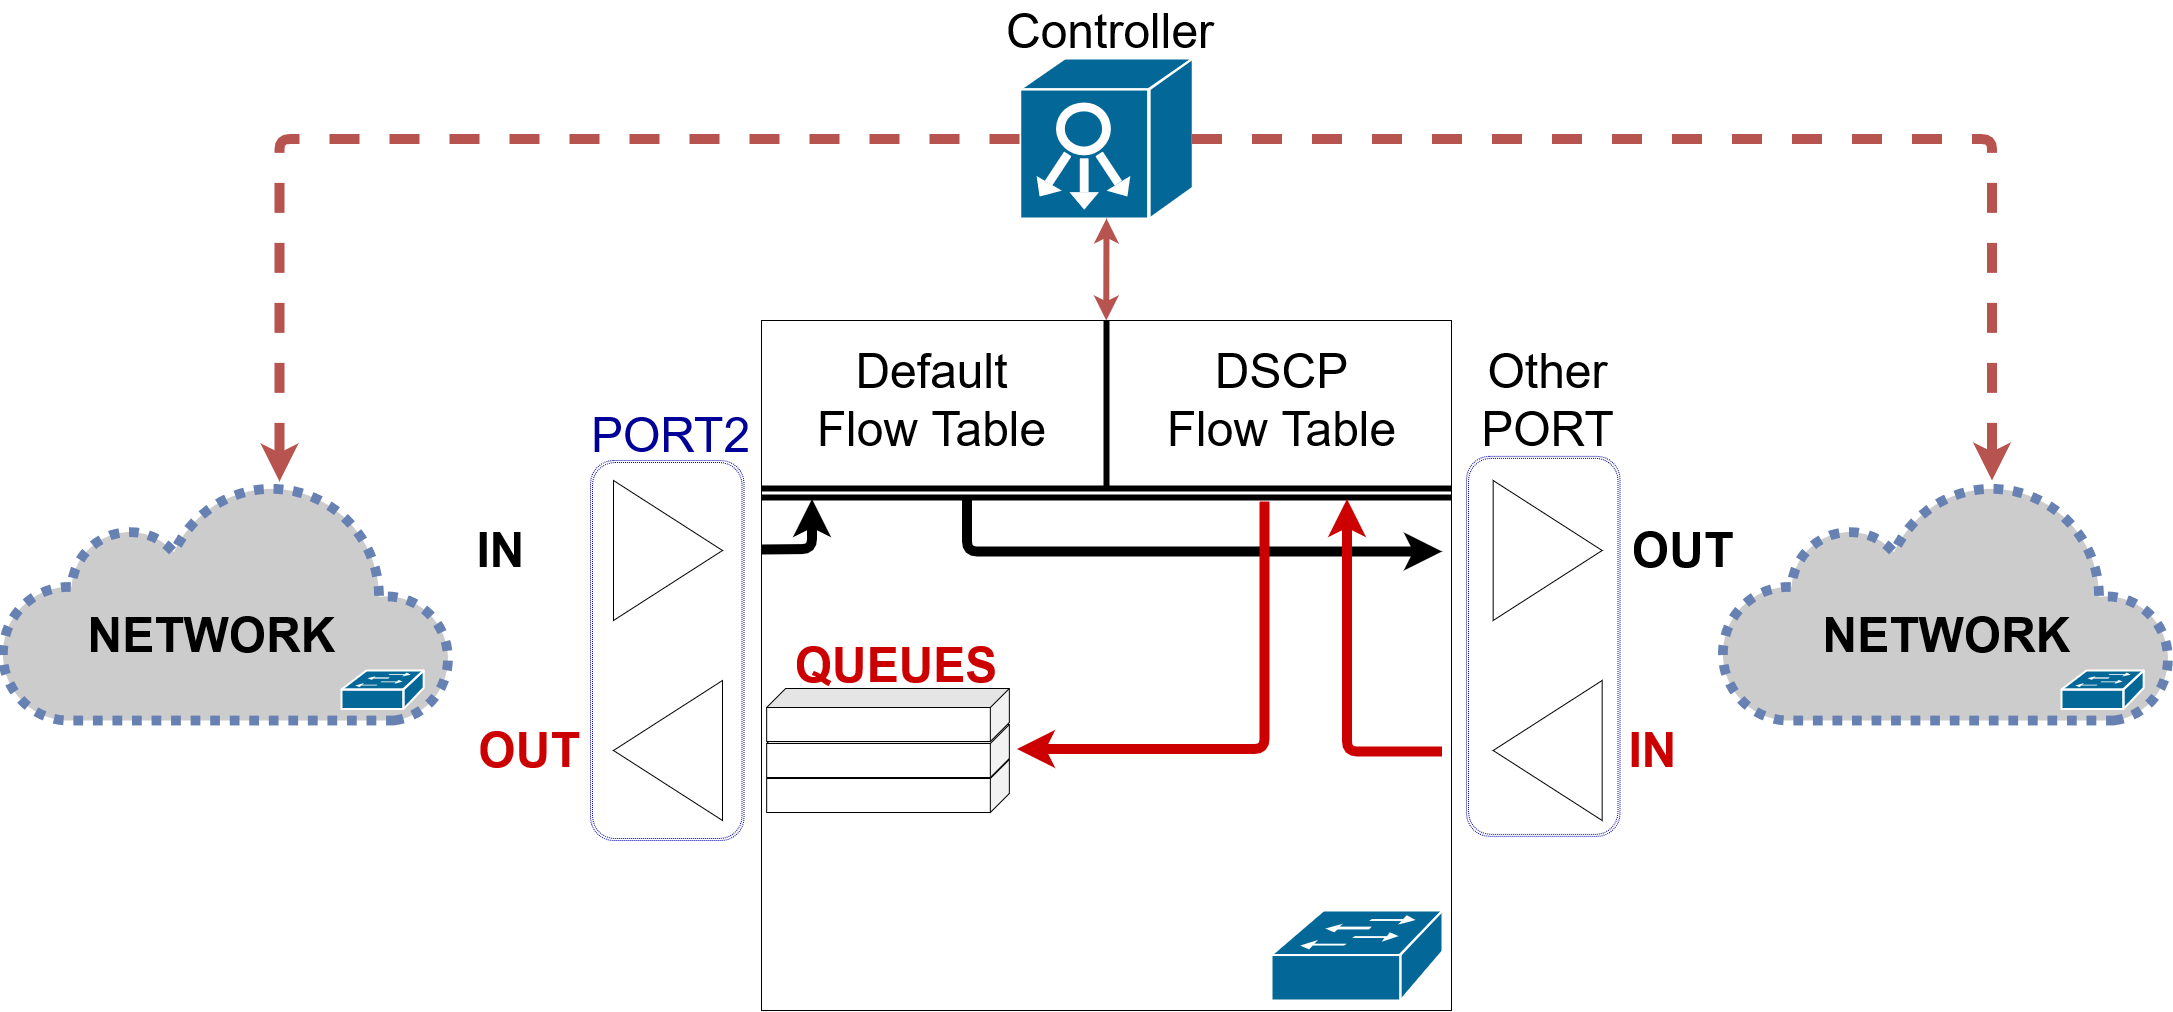
\includegraphics[width=13cm]{figure/SDN_net_LAST.png}
%	\caption{Simulated Network inside Mininet environment.}
%	\label{fig:{Network}}
%\end{figure}

A network architecture as in Figure \ref{fig:{Network}} has been considered, which aims at representing a portion of a larger network where a bottleneck occurs. More precisely, a switch $s0$ with one input port and one output port, and a remote controller \cite{OVS, RYU} that dynamically manages the configuration of the queues of $s0$ has been emulated. The input of $s0$ is fed with more instance of D-ITG generating stochastic traffic, whose mean value follows the pattern of a real data set (where packets are differentiated by their ToS - Type of Service - priority index) extracted from two days logs of a router of a large service provider network. Namely, the original real data set contains traffic of a real network incoming from a source geographic area and terminating in a destination geographic area, and is divided for each value of Differentiated Services Code Point (DSCP) with a sampling time of 5 minutes \cite{Baker1998, Babiarz2006}. DSCP is the modern definition of the Type of Service (ToS) field, in which the first 6 bits are the Differentiated Services field that are in common with ToS field, and the last 2 bits regard explicit congestion notification. The ToS field can specify the priority of a datagram and the request for a low delay addressing, a high throughput or a high reliability service. Following the implementation of many national service provider networks (see e.g. \cite{Notiziario}), the 8 different values of the DSCP has been partitioned in three classes: the \textit{Default} class (DSCPs $0,1,3$), the \textit{Premium} (DSCPs $2,4,6,7$), and the \textit{Gold} class (DSCP $5$): each queue has been assigned to a single queue, associated with a different priority.

%Traffic generation is entrusted to the D-ITG generator which uses informations inside a database created from a real measure that contains the number of packets transmitted and received by a switch. The database fields has been divided for each type of Differentiated Services Code Point (DSCP) with a sampling time of 5 minutes \cite{Baker1998, Babiarz2006}. DSCP is the modern definition of the Type of Service (ToS) field in which the first 6 bits are the Differentiated Services field that are in common with ToS field, and the last 2 bits are the explicit congestion notification. The ToS field can specify the priority of a datagram and the request for a low delay addressing, a high throughput or a high reliability service. Depending on the ToS values, a packet could be placed in a high priority exit queue, or follow a route with latency, throughput and the appropriate reliability for the request.


Using D-ITG Sender and Receiver SW modules it has been possible to establish a connection between networks n1 and n2. In particular, 16 ITG modules have been initialized: 8 for each network, and within each network one for each DSCP index. These modules handle the sampling time interval (5 minutes), the inter-departure time stochastic distribution associated with the packet rate, the packet size stochastic distribution, the IP and port destinations, and the DSCP index. Regarding the controller SW module RYU has been used, which provides software components with well defined Application Programming Interfaces (API) that give the possibility to easily create new network management and control applications. Ryu supports various protocols for managing network devices, such as OpenFlow, Netconf, OF-config, etc. About OpenFlow, Ryu supports fully 1.0, 1.2, 1.3, 1.4, 1.5 and Nicira Extensions. For the used test-bed the 1.3 version has been chosen. In particular, APIs were used for queue control and counter recovery from the switches \cite{ofctlrest,QoS}. The feedback information collected for the purposes of this work are the descriptions of switches, ports and queues, the number of packets received and transmitted on each port of a switch, the packets passing through the flow tables, the packet rate values of each queue and the packets transmitted by each single queue. In summary, the variables associated to the traffic and control signals in the closed-loop architecture are as follows:

\begin{itemize}
	\item $d(k)\in\Real^{10}$ is a measurable disturbance vector, i.e. representing variables that cannot be controlled. The first 8 components $d_1(k),\ldots,d_8(k)$ consist of the number of packets incoming in the switch $s0$ differentiated with respect to the 8 different values of the DSCPs. $d_9(k)$ and $d_{10}(k)$ are proxy variables, i.e. the hours and minutes of the day, which are very useful to the predictive model since traffic dynamics are tightly correlated with them, e.g. they are substantially different between night and day;
	\item $y(k)\in\Real^{3}$ is the measured output vector, i.e. the variables to regulate. They consist of the number of packets outgoing from switch $s0$ differentiated with respect to the corresponding service class: $y_1(k)$ is the Default Queue output, $y_2(k)$ is the Premium Queue output and $y_3(k)$ is the Gold Queue output;
	\item $u(k)\in\Real^{3}$ is the control input vector. Each component corresponds to the queue configuration of each service class: $u_1(k)$ is the Default Queue configuration, i.e. the maximum admitted bandwidth; $u_2(k)$ is the Premium Queue configuration, i.e. the maximum admitted bandwidth; $u_3(k)$ is the Gold Queue configuration, i.e. the minimum admitted bandwidth;
\end{itemize}

\begin{figure}[tb!]
	\centering
	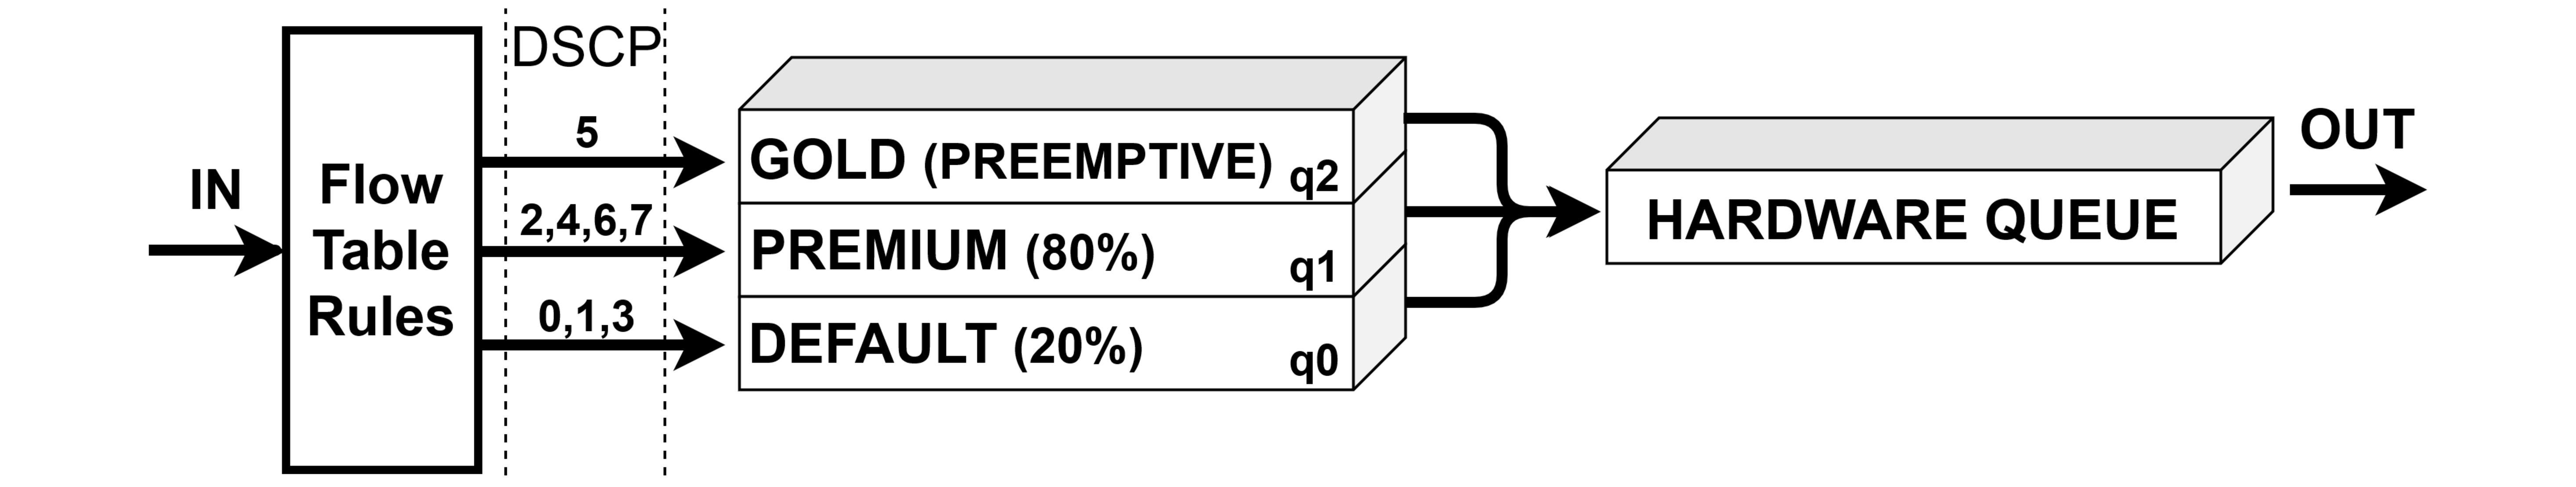
\includegraphics[keepaspectratio,width=\columnwidth]{figure/QUEUE.eps}
%	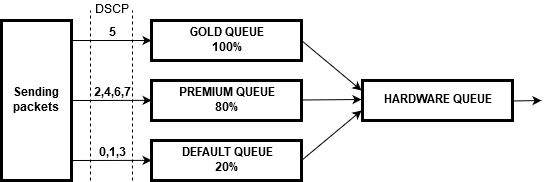
\includegraphics[keepaspectratio,width=12cm]{figure/queue.png}
	\caption{Static queues rate with routed packets relative to DSCP.}
	\label{fig:{queue}}
\end{figure}

In this work the static control of queues used in the Italian service provider network of \textit{Telecom Italia} \cite{Notiziario} has been first applied in the chosen emulative scenario, which is depicted in Figure \ref{fig:{queue}}. To this aim 3 queues in $s0$ and has been defined and configured as follows: packets with the DSCP values 0, 1 and 3 (Default queue) are routed via queue 0, with maximum rate $u_1(k) = 20 \textit{MB/s}, \forall k$; the packets with values 2, 4, 6 and 7 (Premium queue) are routed on queue 1, with maximum rate $u_2(k) = 80 \textit{MB/s}, \forall k$; the packets with value 5 (Gold queue) are routed on queue 2, with minimum rate $u_3(k) = 100 \textit{MB/s}, \forall k$. To obtain this prioritization it has also been necessary to set the flow tables of $s0$ to discriminate incoming packets based on the DSCP value and the destination IP address, and re-route them to the desired queue. Also, to obtain a bottleneck situation in $s0$, the bandwidth of the output port of switch $s0$ has been setted at 100 \textit{MB/s}. Using this configuration queue 2 uses the maximum capacity of the port to forward packets with preemptive priority, while the other two queues use the remaining bandwidth from 0 \textit{MB/s} to the specified maximum bandwidth based on needs.\\
%As formally defined later in Section \ref{secSwitchedModeling}, the packets sent by the queues will be collected in the state vector to be controlled $x(k)\in\mathbf{R}^3,\ \forall k$,  while the bandwidth associated to the queues will compose the control variables vector $u(k)\in\mathbf{R}^3,\ \forall k$.
As will be shown in Section \ref{secExpRes}, using static priority control the queues will not be able to send all the packets incoming from network $n1$, and a dramatic amount of packets will be lost. This motivates the application of optimization techniques, which are enabled by the predictive models derived using the methodology described in the following section.
%\textcolor{blue}{In this work we first applied in our emulative scenario the static control of queues used in the Italian service provider network of \textit{Telecom Italia} \cite{Notiziario}, which is depicted in Figure \ref{fig:{queue}}. To this aim we defined 3 queues in $s0$ and configured the queues as follows: packets with the DSCP values 0, 1 and 3 (Default queue) are routed via queue 0, with maximum rate $u_1(k) = 20 \textit{MB/s}, \forall k$; the packets with values 2, 4, 6 and 7 (Premium queue) are routed on queue 1, with maximum rate $u_2(k) = 80 \textit{MB/s}, \forall k$; the packets with value 5 (Gold queue) are routed on queue 2, with minimum rate $u_3(k) = 100 \textit{MB/s}, \forall k$. To obtain this prioritization it has also been necessary to set the flow tables of $s0$ to discriminate incoming packets based on the DSCP value and the destination IP address, and re-route them to the desired queue. Also, to obtain a bottleneck situation in $s0$, we have chosen the bandwidth of the output port of switch $s0$ at 100 \textit{MB/s}. Using this configuration queue 2 uses the maximum capacity of the port to forward packets with preemptive priority, while the other two queues use the remaining bandwidth from 0 \textit{MB/s} to the specified maximum bandwidth based on needs.\\
%As we will see in Section \ref{secExpRes}, using static priority control the queues will not be able to send all the packets incoming from network $n1$, and a dramatic amount of packets will be lost. This motivates the application of optimization techniques, which are enabled by the predictive models derived using the methodology described in the following section.}

%\begin{figure}[tb!]
%	\centering
%	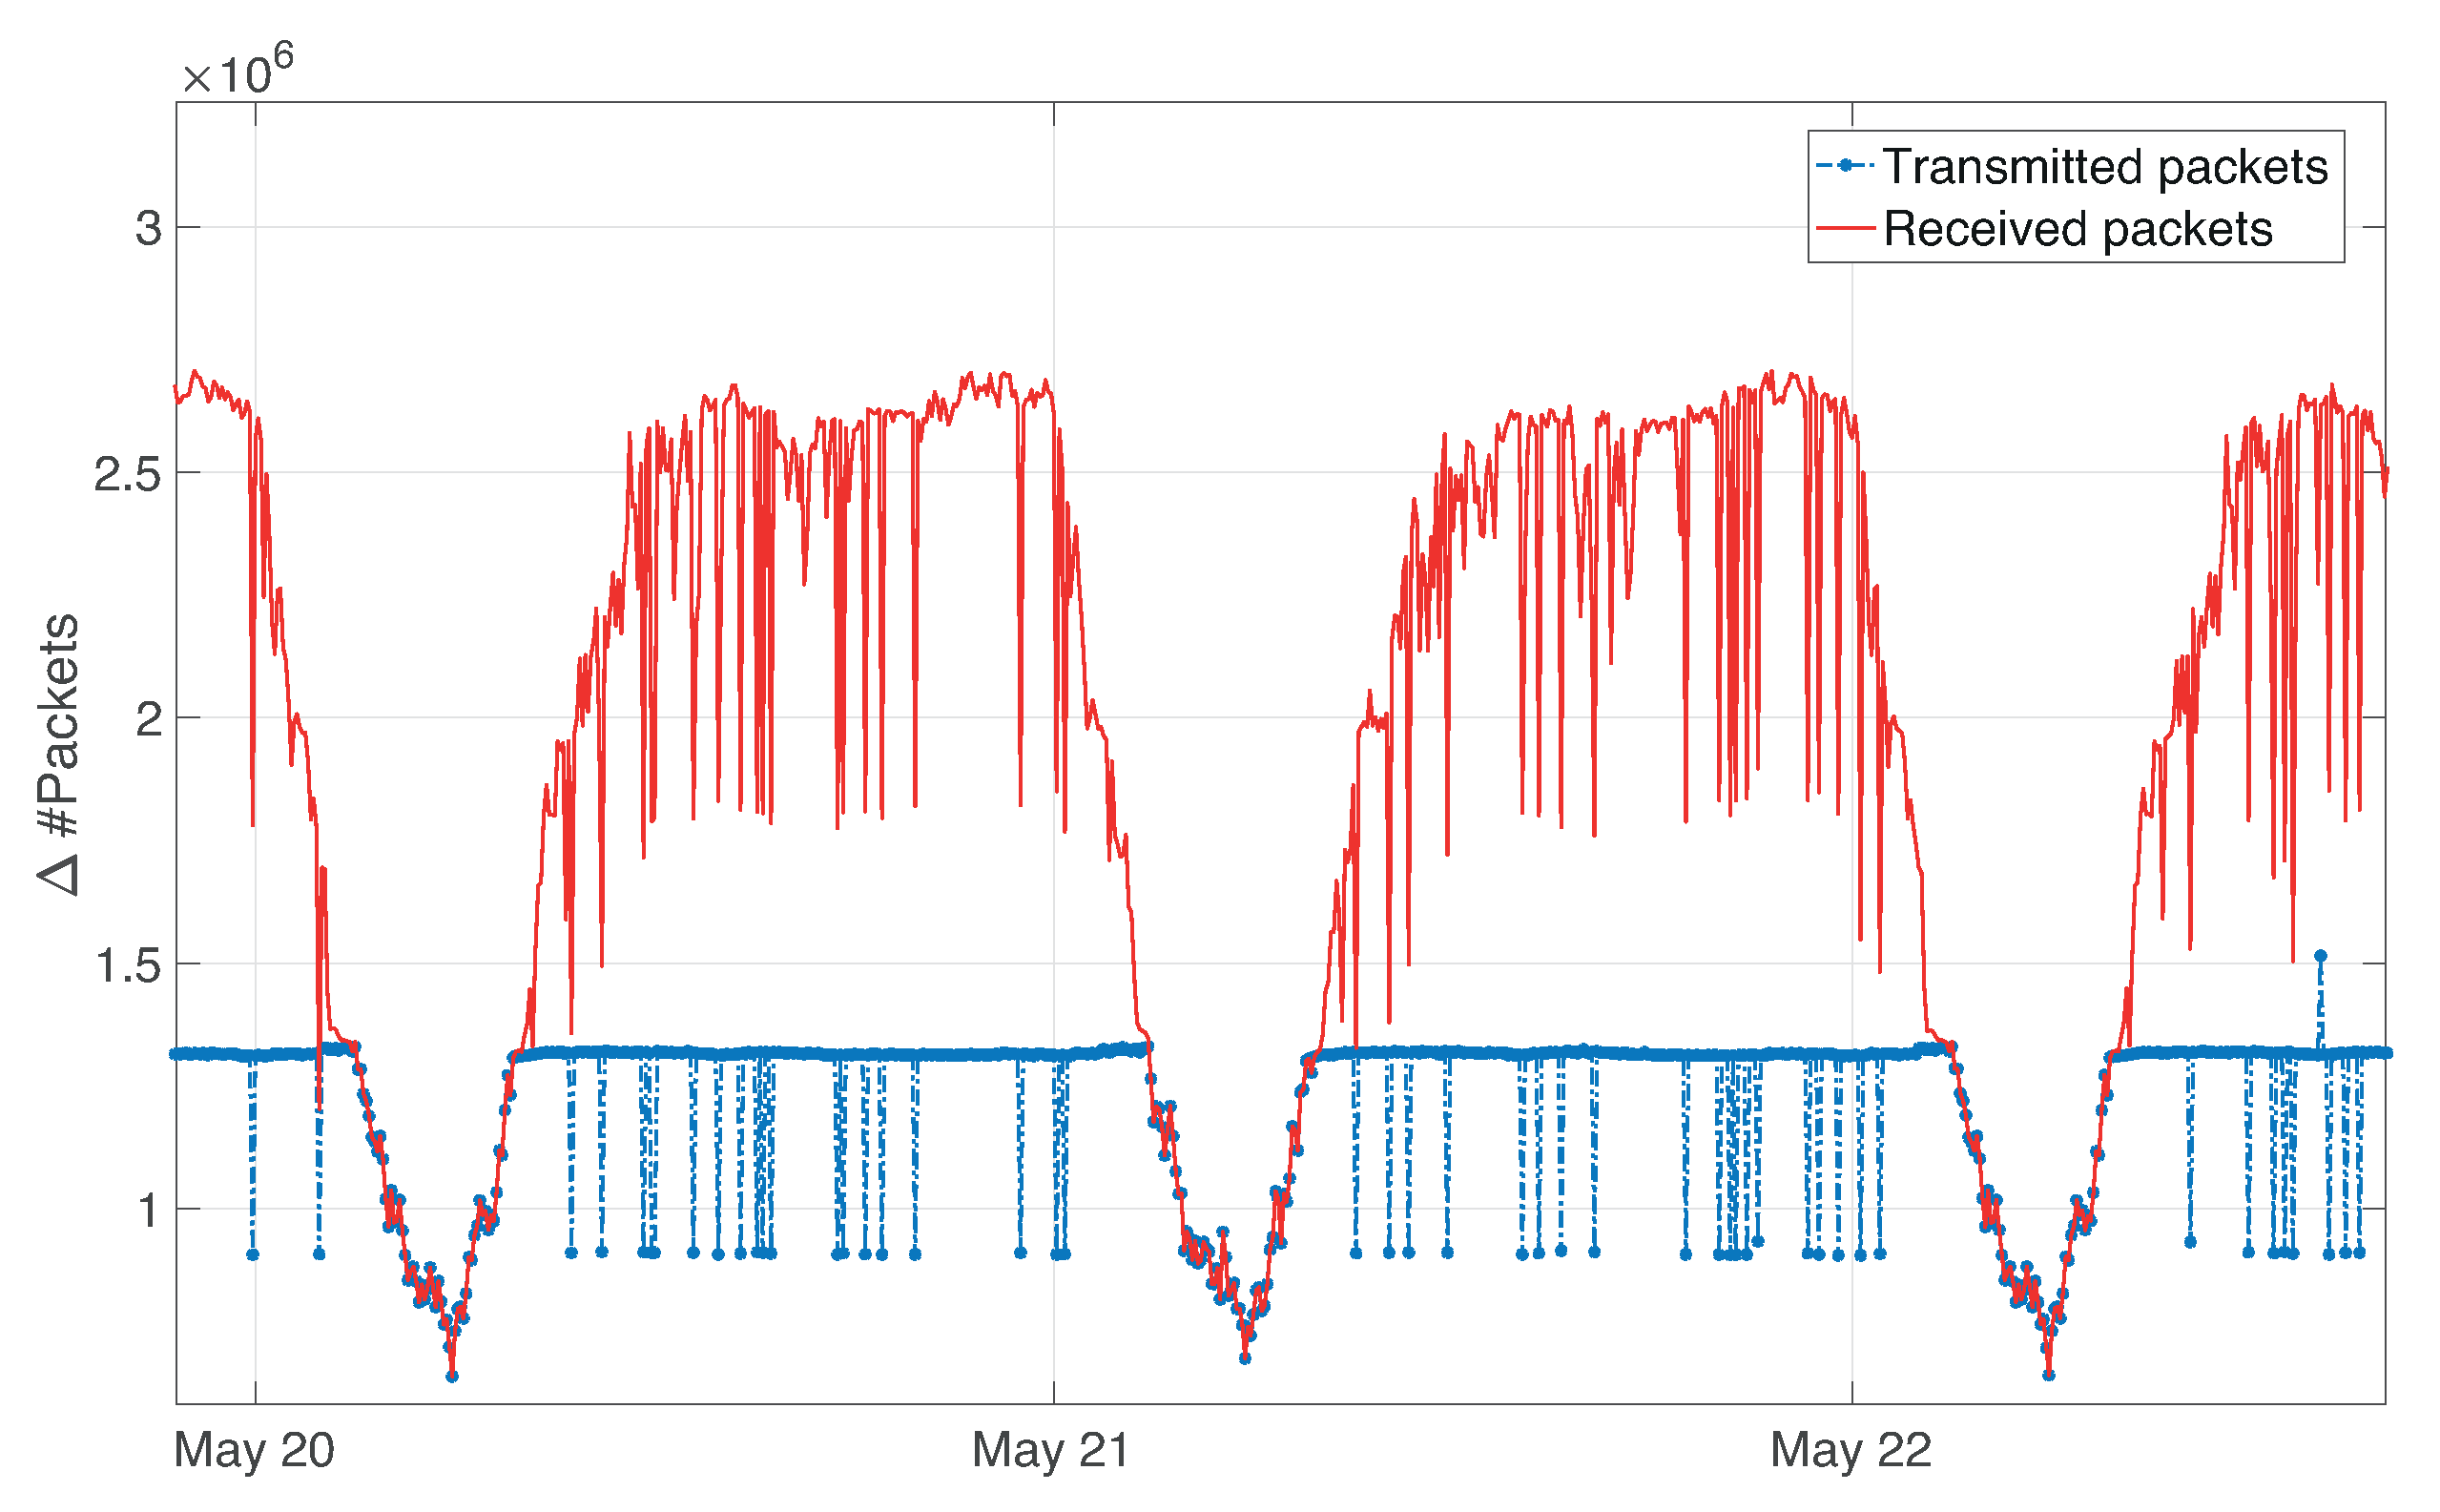
\includegraphics[keepaspectratio,width=\columnwidth]{figure/traffic2Cut.eps}
%	\caption{Received vs. transmitted packets in s0 using static priority as in \cite{Notiziario}.}
%	\label{fig:{Traffic}}
%\end{figure}
%Simulation plots in Figure \ref{fig:{Traffic}} clearly show that using static priority control, as expected, the queues are not able to send all the packets incoming from network n1, and a dramatic amount of packets is lost. This motivates the application of optimisation techniques, which are enabled by the predictive models derived using the methodology described in the following section.


%====================================================================================================
%====================================================================================================